\appendix
\section{Appendices}

\subsection{Simple top design with WRPC}
\label{app:top_design}

\begin{center}
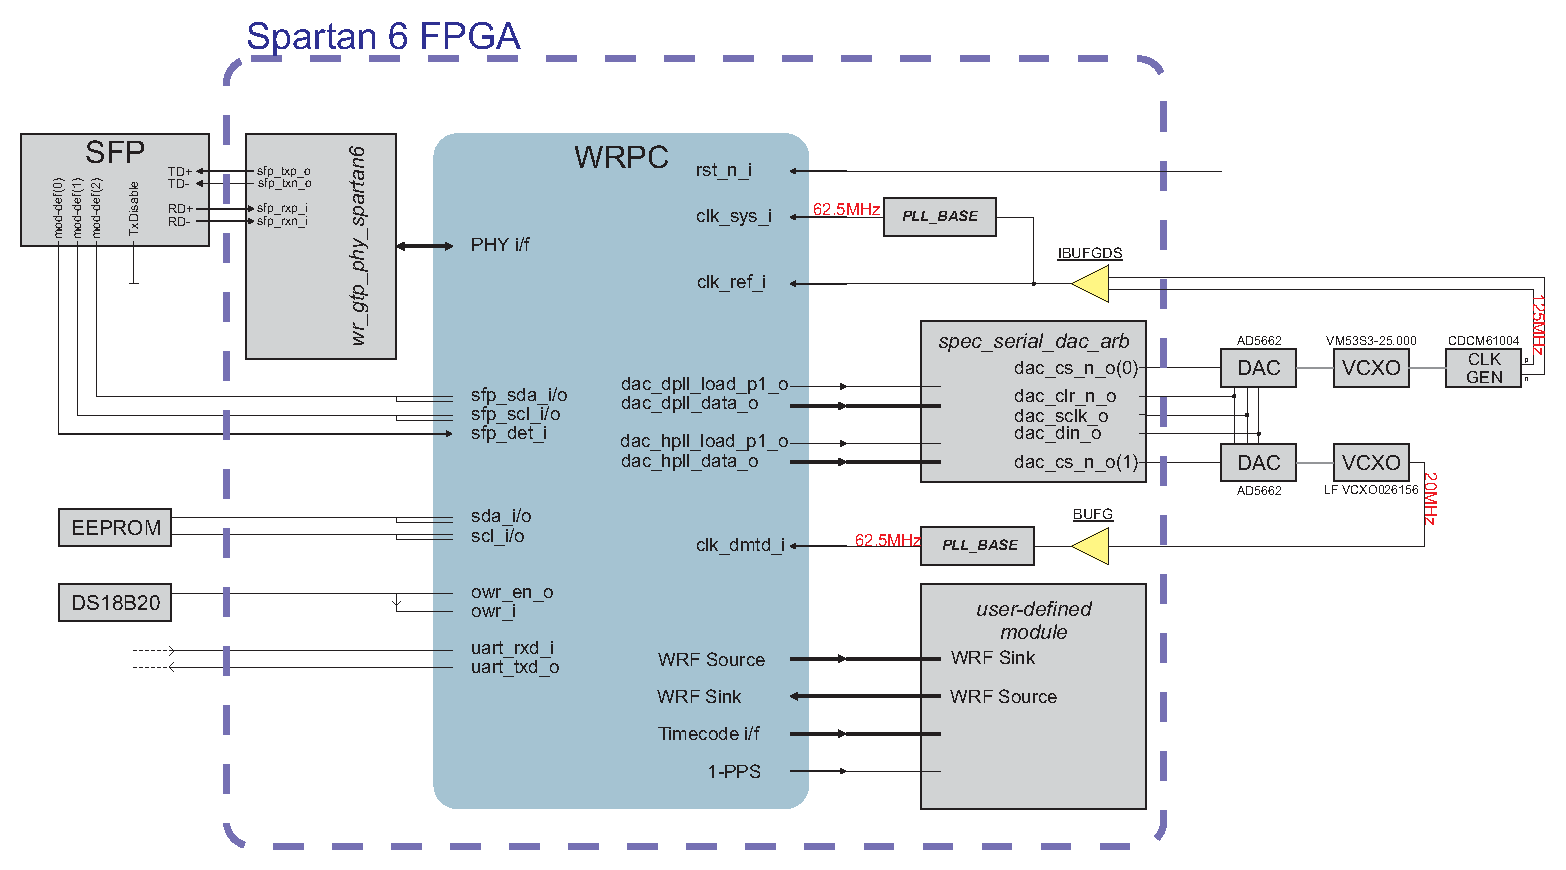
\includegraphics[width=.9\textheight, angle=90]{fig/basic_top.pdf}
\end{center}

%\newpage
%\subsection{WR Fabric testbench example}
%\label{app:fabric_tb}
%
%\begin{lstlisting}
%/* A small testbench demonstrating how to send Ethernet packets 
% * over WRPC's Fabric interface.*/
%
%`include "if_wb_master.svh"
%`include "if_wb_slave.svh"
%`include "wb_packet_sink.svh"
%`include "wb_packet_source.svh"
%
%`timescale 1ns/1ns
%
%module main;
%
%   reg                   clk = 0;
%   reg                   rst = 0;
%
%   /* Clock / reset generation */
%   initial #100 rst = 1;
%   always #10 clk <= ~clk;
%
%   /* Packet Sink Wishbone interface (slave) - inputs packets,
%    * simulating a MAC TX input.*/
%   IWishboneSlave
%     #(
%       .g_data_width(16),
%       .g_addr_width(2))
%   U_WB_Slave
%     (
%      .clk_i(clk),
%      .rst_n_i(rst)
%      );
%
%   /* Packet Sink Wishbone interface (slave) - inputs packets,
%    * simulating a MAC TX input.*/
%   IWishboneMaster
%     #(
%       .g_data_width(16),
%       .g_addr_width(2))
%   U_WB_Master
%     (
%      .clk_i(clk),
%      .rst_n_i(rst)
%      );
%
%   assign U_WB_Slave.adr = U_WB_Master.adr;
%   assign U_WB_Slave.dat_i = U_WB_Master.dat_o;
%   assign U_WB_Slave.cyc = U_WB_Master.cyc;
%   assign U_WB_Slave.stb = U_WB_Master.stb;
%   assign U_WB_Slave.sel = U_WB_Master.sel;
%   assign U_WB_Slave.we = U_WB_Master.we;
%
%   assign U_WB_Master.ack = U_WB_Slave.ack;
%   assign U_WB_Master.stall = U_WB_Slave.stall;
%   assign U_WB_Master.rty = U_WB_Slave.rty;
%   assign U_WB_Master.err = U_WB_Slave.err;
%
%   /* Packet Transmission process */
%   initial begin
%
%      /* Create a Packet Source object: WBPacketSource class
%       * takes Ethernet packets and converts them to 
%       * Wishbone transactions .*/
%      WBPacketSource src = new(U_WB_Master.get_accessor());
%      EthPacket pkt, template = new;
%      EthPacketGenerator gen = new;
%
%      int i;
%
%      /* Force the WB Master to make some mess on the bus by 
%       * throttling transfer rate (random empty slots).*/
%      U_WB_Master.settings.gen_random_throttling = 1;
%      U_WB_Master.settings.throttle_prob = 0.05;
%
%      /* Size range: 64 to 128 bytes */
%      gen.set_size(64, 128);
%
%      /* Payload = sequence of increasing bytes */
%      gen.set_randomization(EthPacketGenerator::SEQ_PAYLOAD);
%
%      template.src = '{ 'hca, 'hfe, 'hba, 'hbe, 'h00, 'h01 };
%      template.dst = '{ 'hff, 'hff, 'hff, 'hff, 'hff, 'hff };
%      template.ethertype = 'h1234;
%
%      /* Set template header for all generated packets 
%       * (i.e. MAC, Ethertype). */
%      gen.set_template(template);
%
%      /* Wait until reset goes low */
%      #200;
%
%      for (i = 0; i < 10; i++) begin
%         pkt = gen.gen();
%         $display("Send %d\n", i);
%         src.send(pkt);
%      end
%   end
%
%   initial begin
%      /* Create a Packet Sink object: WBPacketSink class
%       * decodes Wishbone transactions into Ethernet packets.*/
%      WBPacketSink snk = new (U_WB_Slave.get_accessor());
%      EthPacket pkt;
%
%      int i;
%
%      /* Make the WB Slave sometimes stall the Wishbone link,
%       * to demonstrate various conditions on the bus.*/
%      U_WB_Slave.settings.gen_random_stalls = 1;
%      U_WB_Slave.settings.stall_prob = 0.05;
%      U_WB_Slave.settings.stall_min_duration = 1;
%      U_WB_Slave.settings.stall_max_duration = 5;
%
%      /* Wait until reset goes low */
%      #200;
%
%      /* Print all received packets */
%      forever begin
%         snk.recv(pkt);
%         pkt.dump();
%      end
%   end
%
%endmodule // main
%\end{lstlisting}
